\documentclass{school-22.211-notes}
\date{March 21, 2012}

\begin{document}
\maketitle

\clearpage
\topic{Multi-Group Diffusion Theory}

The diffusion coefficient approximation table is very important: $\frac{1}{3\Sigma_t}$ is off by a factor of 3! 



The group diffusion coefficient $D_g$ should be a tensor; but in application, we assume that $D_g$ is the same for all directions. A more accurate approach is to let $D_g$ be the same in the x-y plane, but different in axial direction. 




\clearpage
\topic{Concepts Derived From Transport Theory}
\subtopic{Applications of Diffusion Theory}
\begin{enumerate}
\item 3D Noval Approach
\item 3D Pin Approach: treat each pin as homogenized; solve 3D homogenized pin few-group diffusion problem. 
\item [FIXME]
\end{enumerate}

\subtopic{Continuity Conditions}


\subtopic{Partial Currents}


\hi{Albedo boundary condition} is the measurement of how much flux is reflected back: 
\eqn{ \alpha = \frac{J^-}{J^+} }


\topic{Boundary Conditions For Diffusion Theory}
In diffusion theory, the incoming partial flux is zero:
\eqn{ J^- = \frac{1}{4} \phi - \frac{1}{2} J_n = 0 }
There are two formulisms to get the boundary condition: 
\begin{enumerate}
\item 
\eqn{ \frac{J}{\phi} = \frac{1}{2} }
\item The more conventional boundary condition is: 
\begin{align}
  J^- &= \frac{1}{4} \phi + \frac{D}{2} \gradient \phi_n \\
  \frac{\gradient \phi}{\phi} &= - \frac{1}{2D} = - \frac{3\Sigma_{tr}}{2} = - \frac{1}{d_{\mathrm{extrap}}}, \mbox{ where } d_{\mathrm{extrap}} = \frac{2}{3} \Sigma_{tr}  = \frac{2}{3 \lambda_{\mathrm{tr}}} 
\end{align}
where $D$ is the property of the material inside, and $\lambda_{tr}$ is transport mean free path. Notice that the exact coefficient in $d_{\mathrm{extrap}}$ may be different. 
\end{enumerate}


\topic{Eigenvalue Problem}
We start from a one-group diffusion equation,
\eqn{ - \divergence D(\vecr) \gradient \phi(\vecr) + \Sigma(\vecr) \phi(\vecr) = \frac{1}{\keff} \nu \Sigma_f(\vecr) \phi(\vecr) }
Assume cross sections do not depend on spatial distribution, 

Rearranging, 

Define \hi{material buckling} 
\eqn{ B^2_m = }
Then we get our \hi{Helmholtz equation}:


For a criticality problem, we can solve find the $B^2$ such that the system is critical. Hence giving geometry, only certain materials would make the system critical; given material, only certain geometries would make the system critical. That is, given a reactor, it would be critical if and only if the material and the geometry satisfy,
\eqn{ B_g^2 = B_m^2} 
and there can only be a solution when $\kinf > 1$ (exception: if there is external source, $\kinf$ can be less than 1 and the system is still critical). 


$DB^2_g$ is the leakage per unit volume per unit flux. Notice $\keff$ does not depend on volume or flux. 


\hi{migration area} $M^2 = \frac{D}{\Sigma_a}$ is a measurement of the amount of travelling before absorption. 


\topic{Simple Geometry Laplacians}
Starting from the Helmholtz equation, we only consider the 1D case (that is, only the $r$ dimension).
\begin{enumerate}
\item Slab $\in  \left[- \frac{L}{2}, \frac{L}{2} \right]$:
  \eqn{ \dphidxn2 + B_g^2 \phi (x) = 0 }
  Solution is in the form of $\phi(x) = A \cos (Bx) + C \sin(Bx)$. BCs: $\phi(\pm L/2) = 0$. Two equations two unknowns, 
  \eqn{ \left[ \begin{array}{cc} \cos(BL/2) & \sin(BL/2) \\ \cos(BL/2) & -\sin(BL/2) \end{array} \right] \left[ \begin{array}{cc} A \\ C \end{array} \right] = 0 }
  Set the determinant to be zero, we get $-2 \cos (BL/2) \sin (BL/2) = 0$. There are two possibilities: 
  
\item Sphere $\in [0, R]$:
  \eqn{ \dphidrn2 + \frac{2}{r} \dphidr B_g^2 \phi(r) = 0 }
\item Infinite cylinder $\in [0, R]$
\item Finite cylinder $r \in [0, R], z \in \left[ -\frac{H}{2}, \frac{H}{2} \right]$. 
\item Parallelepiped $\in \left[ -\frac{L_i}{2}, \frac{L_i}{2} \right]$: 
\end{enumerate}
The lowest node is the only one remains after the source is gone. 






\clearpage
%%%%%%%%%%%%%%%%%%%%%%%%% Qualify Exam Start %%%%%%%%%%%%%%%%%%%%%%%%%%%%
\lecture{Facts For Qualify Exam}
\topic{Basics}
\begin{enumerate}
\item Common units, see Table~\ref{units}.
\begin{table}
  \centering
  \begin{tabular}{|c|c|c|c|} \hline
   $\sigma$ & $\Sigma$ & $\phi = nv$ & $R = \phi \Sigma$  \\ \hline
   $\cm^2$ & $1/\cm$ & $\frac{n}{\cm^2 \s}$ & $\frac{\mathrm{reactions}}{\cm^3 \s}$ \\ \hline
  \end{tabular}
  \caption{Units of Common Terms} \label{units}
\end{table}
\item Fast flux in hydrogen is around $10^{14}$ n/cm$^2$s, and on the order of $10^{12}$n/cm$^2$s for thermal flux. 
\item Average fission neutron energy: 2 MeV; average peak fission energy: 1 MeV; see fission sepctrum. 
\item Core decay heat after 1 day is about 1\% rated. 
\item Constants to know: 1u = 931.5 MeV. 
\item The effect of U238 energy self-shielding is about an effect of 10, that is, going from infinite dilution to U/I = 0.1. 
\end{enumerate}

\topic{Cross Section}
\begin{enumerate}
\item* If the neutron cross section is independent of energy at 0K, at 1200K the cross section would have a 1/v energy shape because of thermal motion. 
  
\item* Resonance absorption cross section dominates resonance scattering cross section most of the time (except U238). 

\item* Fission cross section: U235 fission xs at 0.1 eV and 300K is about 200 barns (200-300 barns); Pu239 fission xs is about 475 barns (380-570 barns). Hence in thermal reactors, Pu absorption should be about twice that of uranium. 

\item Elastic scattering cross section as in Figure~\ref{scatter-xs}
\begin{figure}
  \centering
  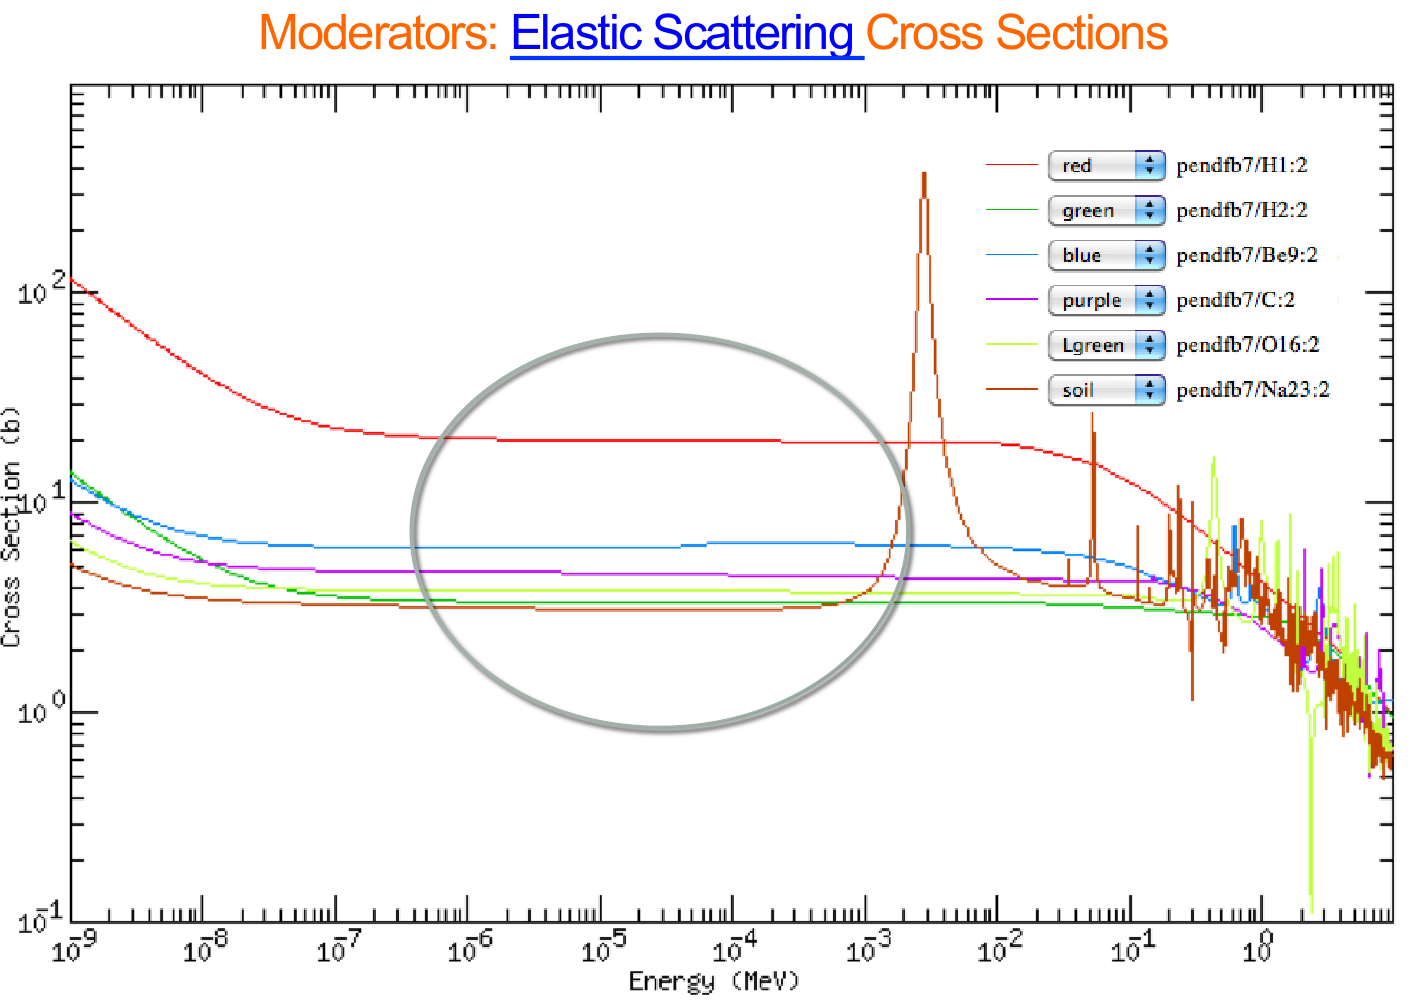
\includegraphics[width=6in]{images/intro/scatter-xs-moderator.png}
  \\
  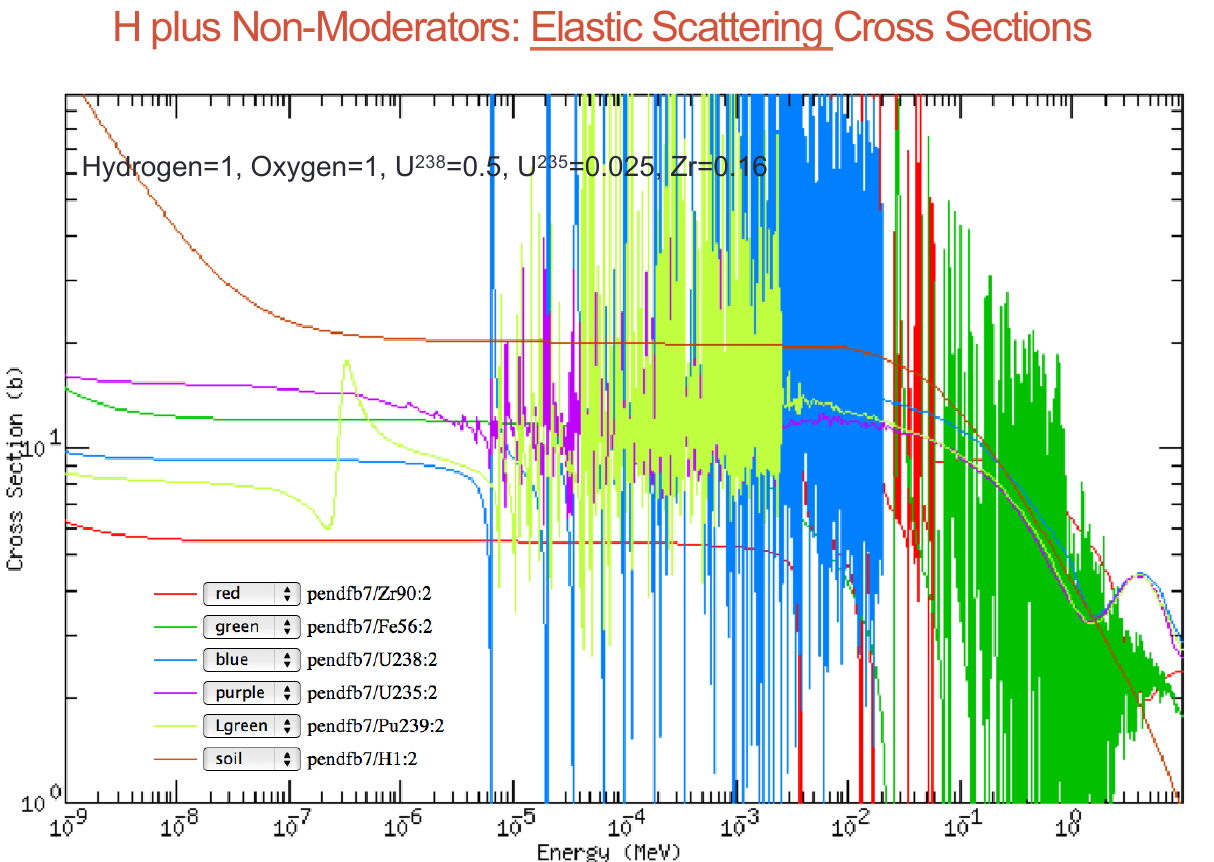
\includegraphics[width=6in]{images/intro/scatter-xs-LWR.png}
  \caption{Elastic Scattering Cross Sections} \label{scatter-xs}
\end{figure}

\item Capture cross section as in Figure~\ref{capture-xs}: 
  \begin{figure}
    \centering
    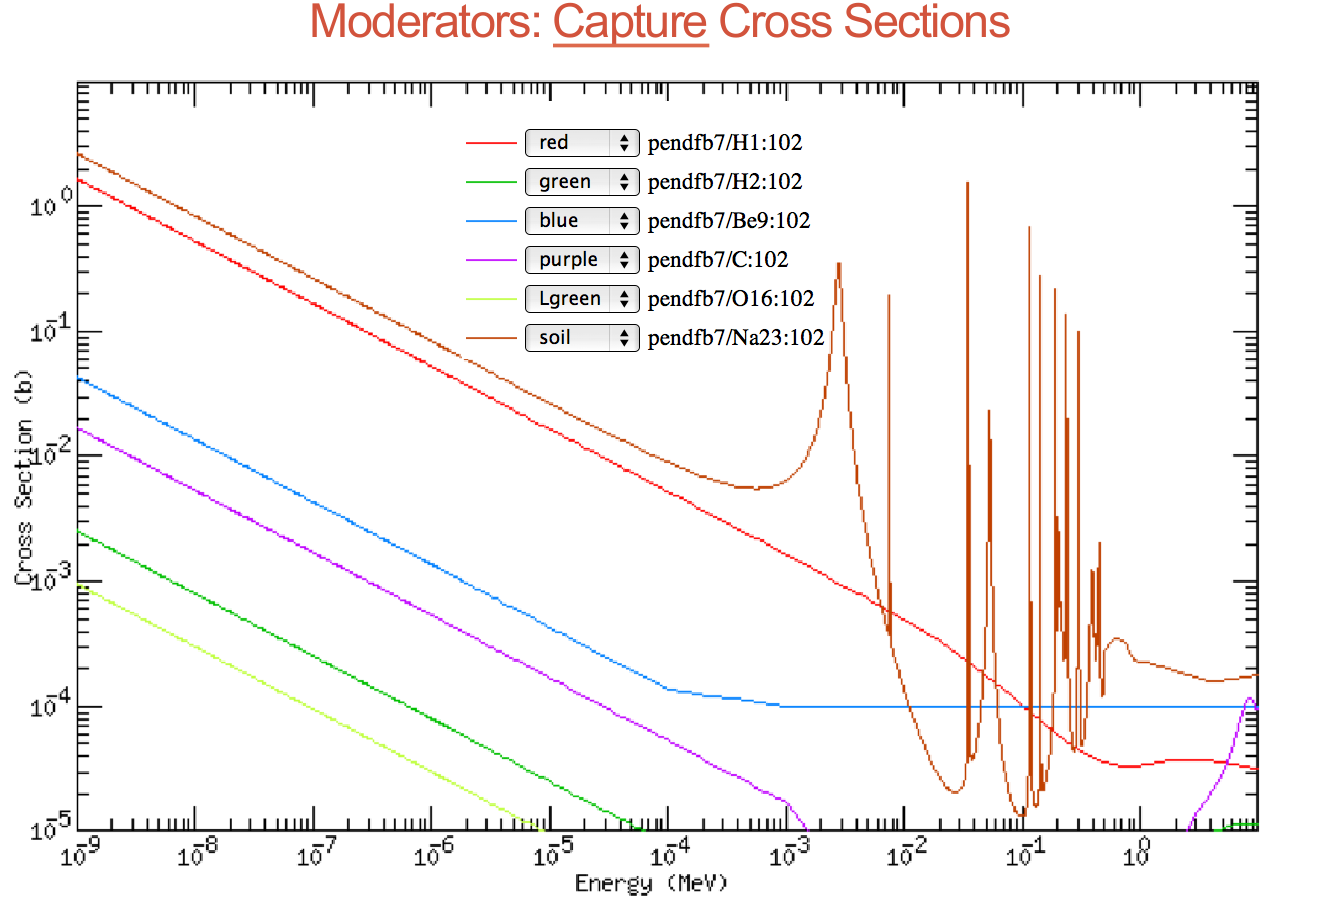
\includegraphics[width=6in]{images/intro/capture-xs.png}
    \\
    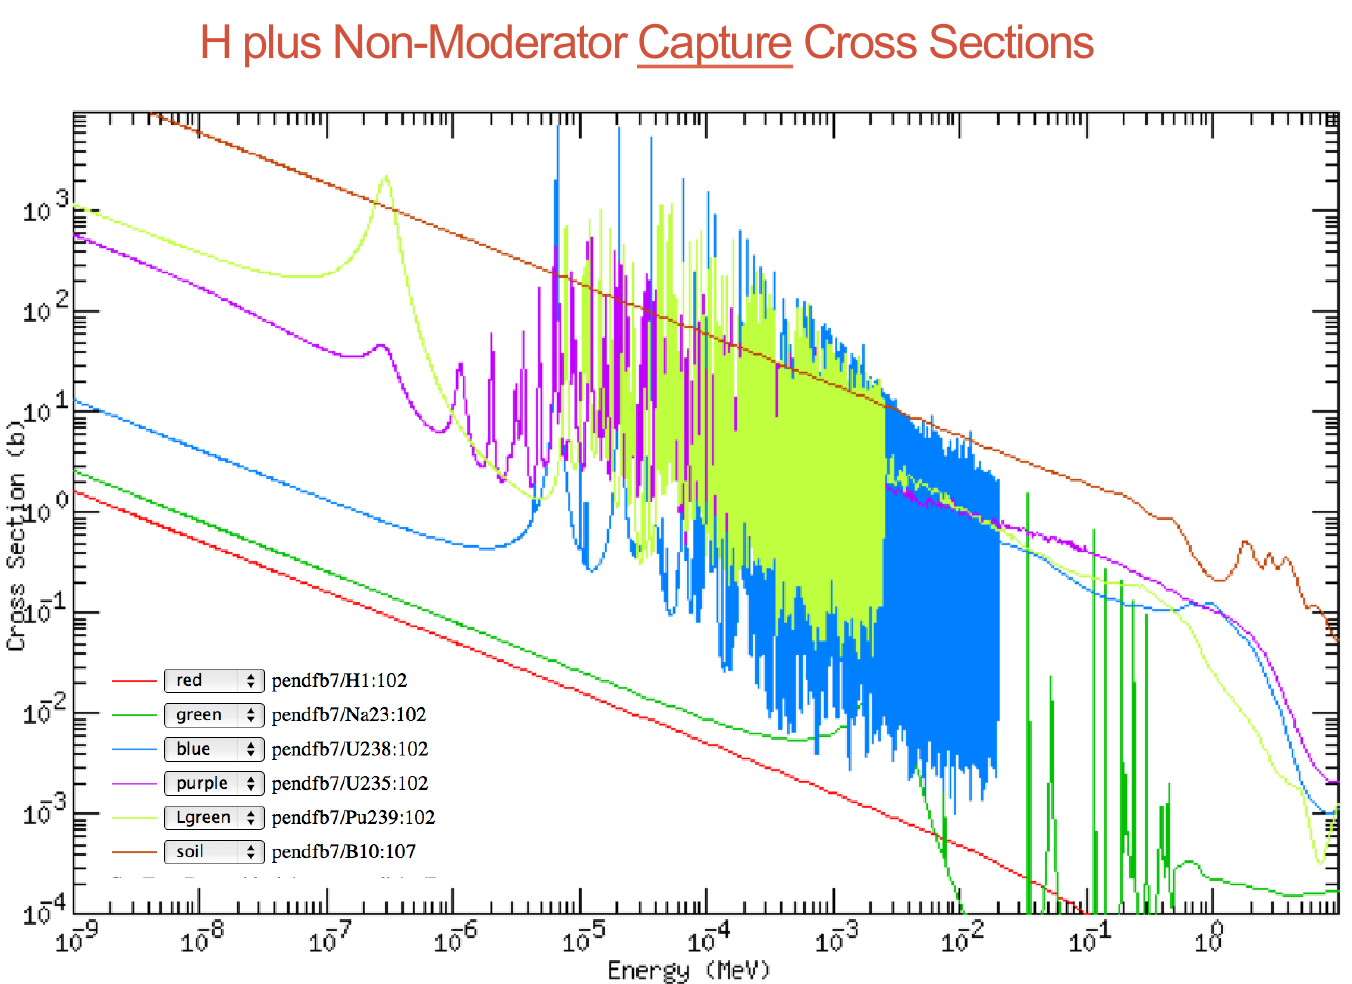
\includegraphics[width=6in]{images/intro/capture-xs-2.png}
    \caption{Capture Cross Section} \label{capture-xs}
  \end{figure}
  \begin{enumerate}
  \item H has no resonance; it has the highest scattering xs in LWR, so we can ignore any other isotopic's neutron scattering.   
  \item Na has a huge resonance in 23 keV, and more resonances at higher energies because it is a heavy isotope.
  \item Near zero energy,
    \eqn{ \sigma(E\to 0) \propto \sqrt{\frac{kT}{AE}}    }
  \item Resonance at 6 to 7 eV: U238. 
  \item U235's thermal elastic xs is larger than 238's, and they both have resonance around the same range.   
  \item A small resonance at .3 eV: Pu239 (its signiture is a super low energy scattering xs). 
  \end{enumerate}

\item Given an unknown material type, all we care is to count the nucleus density of each material and look at it's xs. 
\end{enumerate}

\topic{Kinetics}
\begin{enumerate}
\item PWR 300 pcm/K (Lec10 p. 17, FIXME). 


\item One group k-infinity: in one group $k_{\infty}$ only depends on cross sections $k_{\infty} = \frac{\nu \Sigma_f}{\Sigma_a}$ and has no flux dependency. The flux is buried in the calculation of cross section.
\item Two group k-infinity: we start with neutron balance equation:
\begin{align}
\frac{\nu \Sigma_{f1}}{k_{\infty}} \Phi_1 - \Sigma_{a1} \Phi_1 - \Sigma_{s12} \Phi_1 + \frac{\nu \Sigma_{f2}}{k_{\infty}} \Phi_2 + \Sigma_{s21} \Phi_2 &= 0 \\
\Sigma_{s12} \Phi_1 - \Sigma_{s21} \Phi_2 - \Sigma_{a2} \Phi_2 &= 0 
\end{align}
Typically what we do is to write it in a matrix form and solve for a coupled system. But even better, we can define the \hi{effective removal rate} $\bar{\Sigma}_{s12}$, and re-write the two-group balance equation: 
\begin{align}
\frac{\nu \Sigma_{f1}}{k_{\infty}} \Phi_1 - \Sigma_{a1} \Phi_1 - \bar{\Sigma}_{s12} \Phi_1 + \frac{\nu \Sigma_{f2}}{k_{\infty}} \Phi_2 &= 0 \\
\bar{\Sigma}_{s12} \Phi_1- \Sigma_{a2} \Phi_2 &= 0 
\end{align}
Then we can solve for $\frac{\Phi_1}{\Phi_2}$ from the second equation in terms of cross section, plug in the first equation, and get $k_{\infty}$ from there. Notice that we only know the relative magnitude of $\Phi$ and $\Phi_2$. 

\item Two-group, know $D_1 = 1.5, D_2 = 0.5$. Know Two-group diffusion model on p.26 in Lec11 [FIXME].  

\item Know how the solution forms on p. 18 Lec 11. 
\end{enumerate}
%%%%%%%%%%%%%%%%%%%%%%%%% Qualify Exam End %%%%%%%%%%%%%%%%%%%%%%%%%%%%



\end{document}
